\ifx\allfiles\undefined
\documentclass[8pt a4paper, oneside, UTF8]{ctexbook} 
\usepackage{amsmath}   % 数学公式
\usepackage[dvipsnames]{xcolor}
\usepackage{amsthm}    % 定理环境
\usepackage{amssymb}   % 更多公式符号
\usepackage{graphicx}  % 插图
\usepackage{mathrsfs}  % 数学字体
\usepackage{enumitem}  % 列表
\usepackage{geometry}  % 页面调整
\usepackage{unicode-math}
\usepackage{extarrows}
\usepackage{subfigure}
\usepackage{extarrows}
\usepackage{footnote}
\usepackage{svg}
\usepackage{lmodern}
\usepackage{anyfontsize}
\usepackage[colorlinks,linkcolor=black]{hyperref}
\usepackage{supertabular}
\usepackage{tcolorbox}
\usepackage{ulem}
\usepackage{framed}
\usepackage{float}
\usepackage{microtype}
\newcommand{\arccot}{\mathrm{arccot}\,}
\tcbuselibrary{breakable}
\tcbuselibrary{most}
\newcounter{problemname}

\newenvironment{solution}{\par\noindent\textbf{解答. }}{\par}
\newenvironment{note}{\par\noindent\textbf{题目\arabic{problemname}的注记. }}{\par}
\definecolor{shadecolor}{RGB}{241, 241, 255}
\newenvironment{problem}{\begin{shaded}\stepcounter{problemname}\par\noindent\textbf{题目\arabic{problemname}. }}{\end{shaded}\par}
\allowdisplaybreaks
\graphicspath{ {figure/},{../figure/}, {config/}, {../config/} }  % 配置图形文件检索目录
\linespread{1.5} % 行高

% 页码设置
\geometry{top=25.4mm,bottom=25.4mm,left=20mm,right=20mm,headheight=2.17cm,headsep=4mm,footskip=12mm}

% 设置列表环境的上下间距
\setenumerate[1]{itemsep=5pt,partopsep=0pt,parsep=\parskip,topsep=5pt}
\setitemize[1]{itemsep=5pt,partopsep=0pt,parsep=\parskip,topsep=5pt}
\setdescription{itemsep=5pt,partopsep=0pt,parsep=\parskip,topsep=5pt}

% 定理环境
% ########## 定理环境 start ####################################

% 定义单独编号,其他四个共用一个编号计数 这里只列举了五种,其他可类似定义(未定义的使用原来的也可)
\newtcbtheorem[auto counter, number within=section, list type=subsubsection, list inside=toc]{defn}{定义}
{
    colback=green!5,colframe=green!35!black,fonttitle=\bfseries, title={Comment \thetcbcounter}, list entry={Comment \thetcbcounter\quad}, %标题
    breakable, %支持跨页
    before upper={\parindent10pt\noindent},  % 支持缩进。\noindent:首行不缩进
    % left = 2mm, %文字离线框左边的边距
    % right = 1mm,%同上
    % top = 1mm,%同上
    % bottom = 1mm,%同上
    % arc is angular = 1mm, % 棱角线框
    % sharp corners, % 直角线框
    % enhanced,frame hidden, % 隐藏线框
    % enhanced, drop fuzzy shadow,  % 显示阴影
}
{def}

\newtcbtheorem[auto counter, number within=section, list type=subsubsection, list inside=toc]{lemma}{引理}
{
    colback=SeaGreen!10!CornflowerBlue!10,colframe=RoyalPurple!55!Aquamarine!100!,fonttitle=\bfseries, title={Comment \thetcbcounter}, list entry={Comment \thetcbcounter\quad}, %标题
    breakable, %支持跨页
    before upper={\parindent10pt\noindent},  % 支持缩进。\noindent:首行不缩进
    % left = 2mm, %文字离线框左边的边距
    % right = 1mm,%同上
    % top = 1mm,%同上
    % bottom = 1mm,%同上
    % arc is angular = 1mm, % 棱角线框
    % sharp corners, % 直角线框
    % enhanced,frame hidden, % 隐藏线框
    % enhanced, drop fuzzy shadow,  % 显示阴影
}
{lem}
\newtcbtheorem[auto counter, number within=section, list type=subsubsection, list inside=toc]{them}{定理}
{
    colback=Salmon!20, colframe=Salmon!90!Black,fonttitle=\bfseries, title={Comment \thetcbcounter}, list entry={Comment \thetcbcounter\quad}, %标题
    breakable, %支持跨页
    before upper={\parindent10pt\noindent},  % 支持缩进。\noindent:首行不缩进
    % left = 2mm, %文字离线框左边的边距
    % right = 1mm,%同上
    % top = 1mm,%同上
    % bottom = 1mm,%同上
    % arc is angular = 1mm, % 棱角线框
    % sharp corners, % 直角线框
    % enhanced,frame hidden, % 隐藏线框
    % enhanced, drop fuzzy shadow,  % 显示阴影
}
{them}
\newtcbtheorem[auto counter, number within=section, list type=subsubsection, list inside=toc]{criterion}{注}
{
    colback=CornflowerBlue!10,colframe=RoyalPurple!55!Aquamarine!100!,fonttitle=\bfseries, title={Comment \thetcbcounter}, list entry={Comment \thetcbcounter\quad}, %标题
    breakable, %支持跨页
    before upper={\parindent10pt\noindent},  % 支持缩进。\noindent:首行不缩进
    % left = 2mm, %文字离线框左边的边距
    % right = 1mm,%同上
    % top = 1mm,%同上
    % bottom = 1mm,%同上
    % arc is angular = 1mm, % 棱角线框
    % sharp corners, % 直角线框
    % enhanced,frame hidden, % 隐藏线框
    % enhanced, drop fuzzy shadow,  % 显示阴影
}
{cri}

\newtcbtheorem[auto counter, number within=section, list type=subsubsection, list inside=toc]{corollary}{推论}
{
    colback=Emerald!10,colframe=cyan!40!black,fonttitle=\bfseries, title={Comment \thetcbcounter}, list entry={Comment \thetcbcounter\quad}, %标题
    breakable, %支持跨页
    before upper={\parindent10pt\noindent},  % 支持缩进。\noindent:首行不缩进
    % left = 2mm, %文字离线框左边的边距
    % right = 1mm,%同上
    % top = 1mm,%同上
    % bottom = 1mm,%同上
    % arc is angular = 1mm, % 棱角线框
    % sharp corners, % 直角线框
    % enhanced,frame hidden, % 隐藏线框
    % enhanced, drop fuzzy shadow,  % 显示阴影
}
{cor}
% colback=red!5,colframe=red!75!black

% ######### 定理环境 end  #####################################

% ↓↓↓↓↓↓↓↓↓↓↓↓↓↓↓↓↓ 以下是自定义的命令  ↓↓↓↓↓↓↓↓↓↓↓↓↓↓↓↓

% 用于调整表格的高度  使用 \hline\xrowht{25pt}
\newcommand{\xrowht}[2][0]{\addstackgap[.5\dimexpr#2\relax]{\vphantom{#1}}}

% 表格环境内长内容换行  
\newcommand{\tabincell}[2]{\begin{tabular}{@{}#1@{}}#2\end{tabular}}

% 使用\linespread{1.5} 之后 cases 环境的行高也会改变,重新定义一个 ca 环境可以自动控制 cases 环境行高
\newenvironment{ca}[1][1]{\linespread{#1} \selectfont \begin{cases}}{\end{cases}}
% 和上面一样
\newenvironment{vx}[1][1]{\linespread{#1} \selectfont \begin{vmatrix}}{\end{vmatrix}}

\def\d{\textup{d}} % 直立体 d 用于微分符号 dx
\def\R{\mathbb{R}} % 实数域
\newcommand{\bs}[1]{\boldsymbol{#1}}    % 加粗,常用于向量
\newcommand{\ora}[1]{\overrightarrow{#1}} % 向量

% 数学 平行 符号
\newcommand{\pll}{\kern 0.5em/\kern -0.8em /\kern 0.5em}

% 用于空行\myspace{1} 表示空一行 填 2 表示空两行  
\newcommand{\myspace}[1]{\par\vspace{#1\baselineskip}}

\begin{document}
\begin{sloppypar}
    % \input{../config/cover} 
    \else
    \fi
    \chapter{行列式}
    \section{行列式的定义}
    \begin{defn}{行列式的本质定义(几何定义)}{}
        不妨设$a_{1}$的长度(模)为$l,a_{2}$的长度(模)为$m,a_{1}$与$x$轴正向的夹角为$\alpha,a_{2}$与$x$轴正向的夹角为$\beta$,如下图所示.
    \begin{center}
        \tikzset{every picture/.style={line width=0.75pt}}
        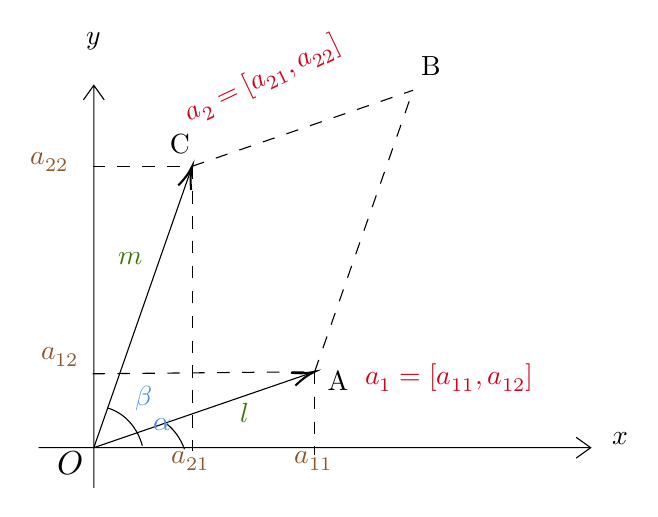
\begin{tikzpicture}[x=0.75pt,y=0.75pt,yscale=-1,xscale=1]        
        \draw  (24,250.6) -- (290,250.6)(50.6,76) -- (50.6,270) (283,245.6) -- (290,250.6) -- (283,255.6) (45.6,83) -- (50.6,76) -- (55.6,83)  ;
        \draw    (50.6,250.6) -- (97.34,116.89) ;
        \draw [shift={(98,115)}, rotate = 109.27] [color={rgb, 255:red, 0; green, 0; blue, 0 }  ][line width=0.75]    (10.93,-3.29) .. controls (6.95,-1.4) and (3.31,-0.3) .. (0,0) .. controls (3.31,0.3) and (6.95,1.4) .. (10.93,3.29)   ;
        \draw    (50.6,250.6) -- (155.11,214.65) ;
        \draw [shift={(157,214)}, rotate = 161.02] [color={rgb, 255:red, 0; green, 0; blue, 0 }  ][line width=0.75]    (10.93,-3.29) .. controls (6.95,-1.4) and (3.31,-0.3) .. (0,0) .. controls (3.31,0.3) and (6.95,1.4) .. (10.93,3.29)   ;
        \draw  [dash pattern={on 4.5pt off 4.5pt}]  (98,115) -- (204.4,78.4) ;
        \draw  [dash pattern={on 4.5pt off 4.5pt}]  (157,214) -- (204.4,78.4) ;
        \draw  [dash pattern={on 4.5pt off 4.5pt}]  (98,115) -- (98,252) ;
        \draw  [dash pattern={on 4.5pt off 4.5pt}]  (50,215) -- (157,214) ;
        \draw  [dash pattern={on 4.5pt off 4.5pt}]  (157,214) -- (157,254) ;
        \draw  [dash pattern={on 4.5pt off 4.5pt}]  (50,115) -- (98,115) ;
        \draw  [draw opacity=0] (57.12,231.43) .. controls (57.53,231.55) and (57.95,231.69) .. (58.37,231.83) .. controls (66.11,234.56) and (71.66,241.33) .. (73.98,249.62) -- (49.71,260.21) -- cycle ; \draw   (57.12,231.43) .. controls (57.53,231.55) and (57.95,231.69) .. (58.37,231.83) .. controls (66.11,234.56) and (71.66,241.33) .. (73.98,249.62) ;  
        \draw  [draw opacity=0] (85.83,239.23) .. controls (89.61,242.25) and (92.51,246.46) .. (94.3,251.33) -- (69.96,265.83) -- cycle ; \draw   (85.83,239.23) .. controls (89.61,242.25) and (92.51,246.46) .. (94.3,251.33) ;  
        \draw (46,49) node [anchor=north west][inner sep=0.75pt]   [align=left] {$\displaystyle y$};
        \draw (32,251) node [anchor=north west][inner sep=0.75pt]  [font=\large] [align=left] {$\displaystyle O$};
        \draw (299,242) node [anchor=north west][inner sep=0.75pt]   [align=left] {$\displaystyle x$};
        \draw (207,61) node [anchor=north west][inner sep=0.75pt]   [align=left] {B};
        \draw (162,212) node [anchor=north west][inner sep=0.75pt]   [align=left] {A};
        \draw (86,98) node [anchor=north west][inner sep=0.75pt]   [align=left] {C};
        \draw (146,251) node [anchor=north west][inner sep=0.75pt]  [color={rgb, 255:red, 139; green, 87; blue, 42 }  ,opacity=1 ] [align=left] {$\displaystyle a_{11}$};
        \draw (87,251) node [anchor=north west][inner sep=0.75pt]  [color={rgb, 255:red, 139; green, 87; blue, 42 }  ,opacity=1 ] [align=left] {$\displaystyle a_{21}$};
        \draw (24,201) node [anchor=north west][inner sep=0.75pt]  [color={rgb, 255:red, 139; green, 87; blue, 42 }  ,opacity=1 ] [align=left] {$\displaystyle a_{12}$};
        \draw (19,107) node [anchor=north west][inner sep=0.75pt]  [color={rgb, 255:red, 139; green, 87; blue, 42 }  ,opacity=1 ] [align=left] {$\displaystyle a_{22}$};
        \draw (61,155) node [anchor=north west][inner sep=0.75pt]  [font=\normalsize,color={rgb, 255:red, 65; green, 117; blue, 5 }  ,opacity=1 ] [align=left] {$\displaystyle m$};
        \draw (120,228) node [anchor=north west][inner sep=0.75pt]  [color={rgb, 255:red, 65; green, 117; blue, 5 }  ,opacity=1 ] [align=left] {$\displaystyle l$};
        \draw (90.88,83.89) node [anchor=north west][inner sep=0.75pt]  [color={rgb, 255:red, 208; green, 2; blue, 27 }  ,opacity=1 ,rotate=-334.49] [align=left] {$\displaystyle a_{2} =[ a_{21} ,a_{22}]$};
        \draw (180,209) node [anchor=north west][inner sep=0.75pt]  [color={rgb, 255:red, 208; green, 2; blue, 27 }  ,opacity=1 ] [align=left] {$\displaystyle a_{1} =[ a_{11} ,a_{12}]$};
        \draw (78,235) node [anchor=north west][inner sep=0.75pt]  [color={rgb, 255:red, 74; green, 144; blue, 226 }  ,opacity=1 ] [align=left] {$\displaystyle \alpha $};
        \draw (74.38,226.9) node  [color={rgb, 255:red, 74; green, 144; blue, 226 }  ,opacity=1 ] [align=left] {$\displaystyle \beta $};
        \end{tikzpicture}
    \end{center}
    那么其围成的平行四边形的面积是:
    $$
    \begin{aligned}
        S_{\square OABC}& =l\cdot m\cdot\sin(\beta-\alpha) \\
        &=l\cdot m(\sin\beta\cos\alpha-\cos\beta\sin\alpha) \\
        &=l\cos\alpha\cdot m\sin\beta-l\sin\alpha\cdot m\cos\beta \\
        &=a_{11}a_{22}-a_{12}a_{21}
    \end{aligned}
    $$
    于是:
    $$
        \begin{vmatrix}a_{11}&a_{12}\\a_{21}&a_{22}\end{vmatrix}=a_{11}a_{22}-a_{12}a_{21}=S_{\square OABC}
    $$
    综上可以得出二阶行列式的几何意义:二阶行列式是由两个二维向量组成的,其(运算规则的)结果为以这两个向量为邻边的平行四边形的面积.\\
    由此可以仿照上述定义可以得到三阶行列式的几何定义为:三阶行列式是由三个三维向量 $a_1=[a_{11},a_{12},a_{13}],a_2=[a_{21},a_{22},a_{23}],a_{3}=[a_{31},a_{32},a_{33}]$组成的,其(运算规则的)结果为以这三个向量为邻边的平行六面体的体积.如下图所示:
    \begin{center}
        \tikzset{every picture/.style={line width=0.75pt}} %set default line width to 0.75pt        
        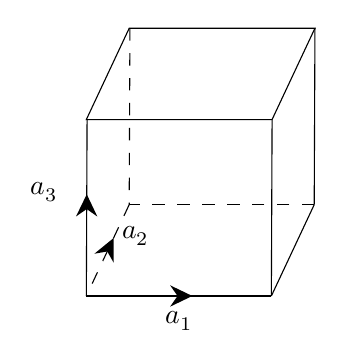
\begin{tikzpicture}[x=0.75pt,y=0.75pt,yscale=-1,xscale=1]
            \draw   (140.65,91) -- (230.14,91) -- (209.49,135) -- (120,135) -- cycle ; 
            \draw    (229.79,176) -- (209.14,220) ; 
            \draw    (230.14,91) -- (229.79,176) ;
            \draw  [dash pattern={on 4.5pt off 4.5pt}]  (229.79,176) -- (140.65,176) ;
            \draw  [dash pattern={on 4.5pt off 4.5pt}]  (140.65,176) -- (120,220) ;
            \draw [shift={(133.09,192.12)}, rotate = 115.14] [fill={rgb, 255:red, 0; green, 0; blue, 0 }  ][line width=0.08]  [draw opacity=0] (10.72,-5.15) -- (0,0) -- (10.72,5.15) -- (7.12,0) -- cycle    ;
            \draw  [dash pattern={on 4.5pt off 4.5pt}]  (141,91) -- (140.65,176) ; 
            \draw    (209.49,135) -- (209.14,220) ;
            \draw    (120.35,135) -- (120,220) ;
            \draw [shift={(120.2,171)}, rotate = 90.23] [fill={rgb, 255:red, 0; green, 0; blue, 0 }  ][line width=0.08]  [draw opacity=0] (10.72,-5.15) -- (0,0) -- (10.72,5.15) -- (7.12,0) -- cycle    ;
            \draw    (209.14,220) -- (120,220) ;
            \draw [shift={(171.07,220)}, rotate = 180] [fill={rgb, 255:red, 0; green, 0; blue, 0 }  ][line width=0.08]  [draw opacity=0] (10.72,-5.15) -- (0,0) -- (10.72,5.15) -- (7.12,0) -- cycle    ;
            \draw (92,164) node [anchor=north west][inner sep=0.75pt]   [align=left] {$\displaystyle a_{3}$};
            \draw (136,185) node [anchor=north west][inner sep=0.75pt]   [align=left] {$\displaystyle a_{2}$};
            \draw (157,226) node [anchor=north west][inner sep=0.75pt]   [align=left] {$\displaystyle a_{1}$};
        \end{tikzpicture}
    \end{center}
    综上,可以得到$n$阶行列式$D_n=
    \begin{vmatrix}
        a_{11} & \cdots &a_{1n}\\ 
        \vdots &        & \vdots\\
        a_{n1} & \cdots & a_{n,n}
    \end{vmatrix}$的本质定义为:
    \textbf{$n$阶行列式是由$n$个$n$维向量$a_1=\begin{bmatrix}a_{11},a_{12},...,a_{1n}\end{bmatrix},a_2=\begin{bmatrix}a_{21},a_{22},...,a_{2n}\end{bmatrix},...,a_n=\begin{bmatrix}a_{n1},a_{n2},...,a_m\end{bmatrix}$组成的,其(运算规则的)结果为以这$n$个向量为邻边的 $n$ 维图形的体积.}\\
    如果把行列式看作是由若干个向量拼成的,并且要把这些向量作运算.以三阶行列式为例,若$D_3 \neq 0$,则意味着体积不为0,则称组成该行列式的三个向量线性无关.若$D_3 =0$\footnote{说明可能存在0向量或者两个向量平行},则称线性相关.
    \end{defn}
    \begin{defn}{行列式的逆序数法定义}{}
    $n(n\geqslant2)$阶行列式:$$\begin{vmatrix}a_{11}&a_{12}&\cdots&a_{1n}\\a_{21}&a_{22}&\cdots&a_{2n}\\\vdots&\vdots&&\vdots\\a_{n1}&a_{n2}&\cdots&a_{nn}\end{vmatrix}=\sum_{j_{1}j_{2}\cdots j_{n}}(-1)^{r(j_{1}j_{2}\cdots j_{n})}a_{1j_{1}}a_{2j_{2}}\cdots a_{nj_{n}}$$
    这里 $\sum_{j_1j_2\cdots j_n} $表示对所有$n$个列下标排列\footnote{排列:由$n$个数$1,2,...,n$组成的一个有序数组称为一个$n$级排列,如$23145$是一个$5$级排列,$41352$也是一个$5$级排列. $n$级排列共有 $n!$ 个.}求和,故为$n!$项之和.注意到行下标已经顺排,而列下标是任一个$n$级排列,\textbf{故每项由取自不同行、不同列的$n$个元素的乘积组成},每项的正、负号取决于$(-1)^{\tau(j_1j_2\cdots j_n)}$.当列下标为奇排列\footnote{逆序:在一个$n$级排列$i_1i_2...i_s...i_r...i_n$中,若$i_s>i_t$,且$i_{s}$排在$i_{t}$前面,则称这两个数构成一个逆序.\\逆序数:一个排列中,逆序的总数称为该排列的逆序数,记作 $\tau(i_1i_2\cdots i_n)$,如 $\tau(231546)=3$ , $\tau(621534)=8$.由小到大顺排的排列称为自然排序,如 12345,显然,自然排序的逆序数为 0.\\奇排列和偶排列:排列的逆序数为奇数时,该排列称为奇排列;排列的逆序数为偶数时,该排列称为偶排列.}时,应附加负号;当列下标为偶排列时,应附加正号.
    \end{defn}
    \begin{defn}{行列式的展开定理定义}{}
        \begin{enumerate}
            \item 余子式:在$n$阶行列式中,去掉元素$a_{ij}$所在的第$i$行、第$j$ 列元素,由剩下的元素按原来的位置与顺序组成的$n-1$ 阶行列式称为元素$a_{ij}$的余子式,记作$M_{ij}$,即
            $$
                \begin{gathered}M_{ij}=\begin{vmatrix}a_{11}&\cdots&a_{1,j-1}&a_{1,j+1}&\cdots&a_{1n}\\\vdots&&\vdots&\vdots&&\vdots\\a_{i-1,1}&\cdots&a_{i-1,j-1}&a_{i-1,j+1}&\cdots&a_{i-1,n}\\a_{i+1,1}&\cdots&a_{i+1,j-1}&a_{i+1,j+1}&\cdots&a_{i+1,n}\\\vdots&&\vdots&\vdots&&\vdots\\a_{n!}&\cdots&a_{n,j-1}&a_{n,j+1}&\cdots&a_{nn}\end{vmatrix}.\end{gathered}
                $$
            \item 代数余子式:余子式$M_{ij}$乘(-1)$^{i+j}$后称为$a_{ij}$的代数余子式,记作$A_{ij}$,即$$A_{ij}=(-1)^{i+j}M_{ij}$$显然也有$M_{ij}=(-1)^{i+j}A_{ij}$
            \item 行列式按某一行展开:行列式的值等于行列式的某行(列)元素分别乘其相应的代数余子式后再求和,即\footnote{目的:降阶,即$n$阶降成$n$个$n-1$阶.展开原则:某一行(列)为$0$的元素越多越好}
            $$
                |A|=\begin{cases}a_{i1}A_{i1}+a_{i2}A_{i2}+\cdots+a_{in}A_{in}=\sum_{j=1}^{n}a_{ij}A_{ij}\left(i=1,2,\cdots,n\right),\\a_{1j}A_{1j}+a_{2j}A_{2j}+\cdots+a_{nj}A_{nj}=\sum_{i=1}^{n}a_{ij}A_{ij}\left(j=1,2,\cdots,n\right).\end{cases}
            $$
        \end{enumerate}
    \end{defn}
    \begin{criterion}{几种特殊的行列式}{}
        \begin{enumerate}
            \item 主对角线行列式(上下三角形行列式):$$\begin{vmatrix}a_{11}&a_{12}&\cdots&a_{1n}\\0&a_{22}&\cdots&a_{2n}\\\vdots&\vdots&&\vdots\\0&0&\cdots&a_{nn}\end{vmatrix}=\begin{vmatrix}a_{11}&0&\cdots&0\\a_{21}&a_{22}&\cdots&0\\\vdots&\vdots&&\vdots\\a_{n1}&a_{n2}&\cdots&a_{nn}\end{vmatrix}=\begin{vmatrix}a_{11}&0&\cdots&0\\0&a_{22}&\cdots&0\\\vdots&\vdots&&\vdots\\0&0&\cdots&a_{nn}\end{vmatrix}=\prod_{i=1}^na_{ii} .$$
            \item 副对角线行列式:$$\begin{vmatrix}a_{11}&\cdots&a_{1,n-1}&a_{1n}\\a_{21}&\cdots&a_{2,n-1}&0\\\vdots&&\vdots&\vdots\\a_{n1}&\cdots&0&0\end{vmatrix}=\begin{vmatrix}0&\cdots&0&a_{1n}\\0&\cdots&a_{2,n-1}&a_{2n}\\\vdots&&\vdots&\vdots\\a_{n1}&\cdots&a_{n,n-1}&a_{nn}\end{vmatrix}=\begin{vmatrix}0&\cdots&0&a_{1n}\\0&\cdots&a_{2,n-1}&0\\\vdots&&\vdots&\vdots\\a_{n1}&\cdots&0&0\end{vmatrix} $$=$(-1)^{\frac{n(n-1)}{2}}a_{1n}a_{2,n-1}\cdots a_{n1}$
            \item 拉普拉斯行列式:设$A$为$m$阶矩阵,$B$为$n$阶矩阵,则:$$\begin{gathered}\begin{vmatrix}A&O\\O&B\end{vmatrix}=\begin{vmatrix}A&C\\O&B\end{vmatrix}=\begin{vmatrix}A&O\\C&B\end{vmatrix}=\begin{vmatrix}A\end{vmatrix}\begin{vmatrix}B\end{vmatrix},\\\begin{vmatrix}O&A\\B&O\end{vmatrix}=\begin{vmatrix}C&A\\B&O\end{vmatrix}=\begin{vmatrix}O&A\\B&C\end{vmatrix}=(-1)^{mn}\begin{vmatrix}A\end{vmatrix}\begin{vmatrix}B\end{vmatrix} .\end{gathered}$$
            \item 范德蒙德行列式\footnote{以三阶范德蒙行列式$\left.\left|\begin{array}{cccc}1&1&1\\\\x_1&x_2&x_3\\\\x_1^2&x_2^2&x_3^2\end{array}\right.\right|$为例,该行列式的值为$(x_3-x_2)(x_2-x_1)$}:$$\begin{vmatrix}1&1&\cdots&1\\x_1&x_2&\cdots&x_n\\x_1^2&x_2^2&\cdots&x_n^2\\\vdots&\vdots&&\vdots\\x_1^{n-1}&x_2^{n-1}&\cdots&x_n^{n-1}\end{vmatrix}=\prod_{1\leqslant i<j\leqslant n}(x_j-x_i).$$
        \end{enumerate}
    \end{criterion}
    \section{行列式的性质}
    \begin{enumerate}
        \item 行列互换,其值不变,即$|A|=|A^T|$,即$ \begin{vmatrix}a_{11}&a_{12}\\a_{21}&a_{22}\end{vmatrix}=a_{11}a_{22}-a_{12}a_{21}= \begin{vmatrix}a_{11}&a_{21}\\a_{12}&a_{22}\end{vmatrix}=a_{11}a_{22}-a_{12}a_{21}$.该条性质说明了 \textcolor{red}{行列式行列等价}
        \\几何解释:很显然平行四边形两条邻边互换,它的面积依然不变.如下图所示:
        \begin{center}
            \tikzset{every picture/.style={line width=0.75pt}} %set default line width to 0.75pt        
                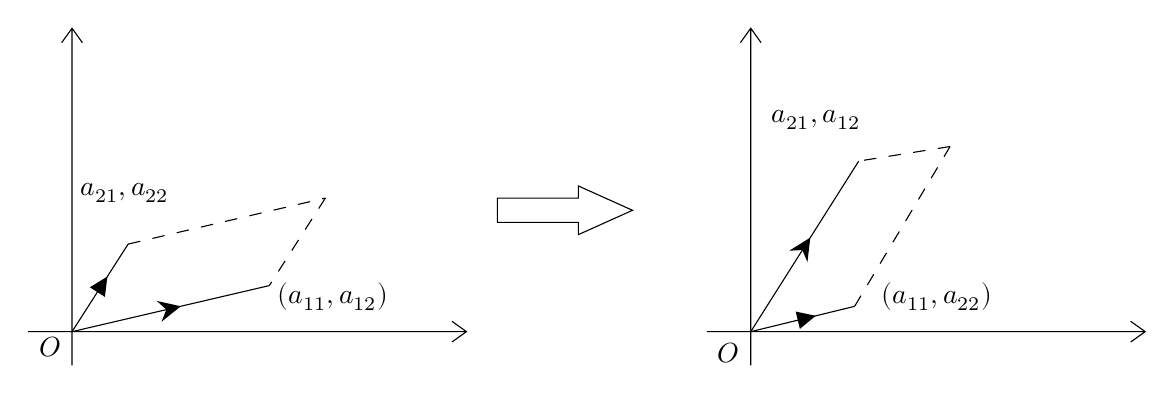
\begin{tikzpicture}[x=0.75pt,y=0.75pt,yscale=-1,xscale=1]
                    \draw  (30,249.76) -- (241.14,249.76)(51.11,103.57) -- (51.11,266) (234.14,244.76) -- (241.14,249.76) -- (234.14,254.76) (46.11,110.57) -- (51.11,103.57) -- (56.11,110.57)  ;
                    \draw    (51.11,249.76) -- (146.14,227.57) ;
                    \draw [shift={(103.5,237.53)}, rotate = 166.86] [fill={rgb, 255:red, 0; green, 0; blue, 0 }  ][line width=0.08]  [draw opacity=0] (10.72,-5.15) -- (0,0) -- (10.72,5.15) -- (7.12,0) -- cycle;
                    \draw    (78.14,207.57) -- (51.11,249.76) ;
                    \draw [shift={(68.14,223.19)}, rotate = 122.65] [fill={rgb, 255:red, 0; green, 0; blue, 0 }  ][line width=0.08]  [draw opacity=0] (8.93,-4.29) -- (0,0) -- (8.93,4.29) -- cycle    ;
                    \draw  [dash pattern={on 4.5pt off 4.5pt}]  (78.14,207.57) -- (173.17,185.39) ;
                    \draw  [dash pattern={on 4.5pt off 4.5pt}]  (173.17,185.39) -- (146.14,227.57) ;
                    \draw   (256,185.43) -- (295.09,185.43) -- (295.09,179.57) -- (321.14,191.29) -- (295.09,203) -- (295.09,197.14) -- (256,197.14) -- cycle ; 
                    \draw  (357,249.76) -- (568.14,249.76)(378.11,103.57) -- (378.11,266) (561.14,244.76) -- (568.14,249.76) -- (561.14,254.76) (373.11,110.57) -- (378.11,103.57) -- (383.11,110.57)  ;
                    \draw    (378.11,249.76) -- (430.14,167.57) ;
                    \draw [shift={(406.8,204.44)}, rotate = 122.34] [fill={rgb, 255:red, 0; green, 0; blue, 0 }  ][line width=0.08]  [draw opacity=0] (10.72,-5.15) -- (0,0) -- (10.72,5.15) -- (7.12,0) -- cycle    ;
                    \draw    (428.14,237.57) -- (378.11,249.76) ;
                    \draw [shift={(409.44,242.13)}, rotate = 166.31] [fill={rgb, 255:red, 0; green, 0; blue, 0 }  ][line width=0.08]  [draw opacity=0] (8.93,-4.29) -- (0,0) -- (8.93,4.29) -- cycle    ;
                    \draw  [dash pattern={on 4.5pt off 4.5pt}]  (428.14,237.57) -- (474.14,160.57) ;
                    \draw  [dash pattern={on 4.5pt off 4.5pt}]  (474.14,160.57) -- (430.14,167.57) ;
                    \draw (149,225) node [anchor=north west][inner sep=0.75pt]   [align=left] {$\displaystyle ( a_{11} ,a_{12})$};
                    \draw (54,177) node [anchor=north west][inner sep=0.75pt]  [font=\normalsize] [align=left] {$\displaystyle \mathnormal{a_{21} ,a_{22}}$};
                    \draw (440,225) node [anchor=north west][inner sep=0.75pt]   [align=left] {$\displaystyle ( a_{11} ,a_{22})$};
                    \draw (387,142) node [anchor=north west][inner sep=0.75pt]  [font=\normalsize] [align=left] {$\displaystyle \mathnormal{a_{21} ,a_{12}}$};
                    \draw (34,251) node [anchor=north west][inner sep=0.75pt]   [align=left] {$\displaystyle O$};
                    \draw (361,254) node [anchor=north west][inner sep=0.75pt]   [align=left] {$\displaystyle O$};
                \end{tikzpicture}
        \end{center}
        \item 若行列式中某行(列)元素全为零,则行列式为零\\
        几何解释:以二阶行列式为例:一个向量无法组成面积,因此如果二阶行列式某行某列全为0的话,无法组成面积.
        \item 若行列式中某行(列)元素有公因子$k(k \neq 0)$,则$k$可提到行列式外面,即
        $$\begin{vmatrix}a_{11}&a_{12}&\cdots&a_{1n}\\\vdots&\vdots&&\vdots\\ka_{i1}&ka_{i2}&\cdots&ka_{in}\\\vdots&\vdots&&\vdots\\a_{n1}&a_{n2}&\cdots&a_{nn}\end{vmatrix}=k\begin{vmatrix}a_{11}&a_{12}&\cdots&a_{1n}\\\vdots&\vdots&&\vdots\\a_{i1}&a_{i2}&\cdots&a_{in}\\\vdots&\vdots&&\vdots\\a_{n1}&a_{n2}&\cdots&a_{nn}\end{vmatrix}$$
        如果行列式某行元素都乘上了$k$倍,以二阶行列式为例,说明这个边乘上了$k$倍,在图像面积上就是整个二阶行列式的面积乘上了$k$倍.
        \item 行列式中某行(列)元素均是两个元素之和,则可拆成两个行列式之和,即
        $$\begin{vmatrix}a_{11}&a_{12}&\cdots&a_{1n}\\\vdots&\vdots&&\vdots\\a_{i1}+b_{i1}&a_{i2}+b_{i2}&\cdots&a_{in}+b_{in}\\\vdots&\vdots&&\vdots\\a_{n1}&a_{n2}&\cdots&a_{nn}\end{vmatrix}=\begin{vmatrix}a_{11}&a_{12}&\cdots&a_{1n}\\\vdots&\vdots&&\vdots\\a_{i1}&a_{i2}&\cdots&a_{in}\\\vdots&\vdots&&\vdots\\a_{n1}&a_{n2}&\cdots&a_{nn}\end{vmatrix}+\begin{vmatrix}a_{11}&a_{12}&\cdots&a_{1n}\\\vdots&\vdots&&\vdots\\b_{i1}&b_{i2}&\cdots&b_{in}\\\vdots&\vdots&&\vdots\\a_{n1}&a_{n2}&\cdots&a_{nn}\end{vmatrix}$$
        该性质又叫行列式的单行(列)可拆性,说明行列式可以拆为两个行列式的和.
        \item 行列式中两行(列)互换,行列式的值反号.\\
        以二阶行列式为例,两行两列互换,则夹角改变,即从$\sin(\beta-\alpha) \rightarrow \sin(\alpha-\beta)$
        \item 行列式中的两行(列)元素相等或对应成比例,则行列式为零.\\
        以二阶行列式为例,行列式两行元素相等或者两行元素成比例,说明两个向量重合或者平行,那么无法组成面积.
        \item 行列式中某行(列)的,倍加到另一行(列),行列式的值不变.
        \begin{proof}[行列式性质$7$证明]
            以二阶行列式为例:
            $$
            \begin{vmatrix}
                a_{11} & a_{12}\\
                a_{21} & a_{22}
            \end{vmatrix}=\begin{vmatrix}
                a_{11} & a_{12}\\
                a_{21}+ka_{11} & a_{22}+ka_{12}
            \end{vmatrix}=\begin{vmatrix}
                a_{11} & a_{12}\\
                a_{21} & a_{22}
            \end{vmatrix}+\begin{vmatrix}
                a_{11} & a_{12}\\
                ka_{11} & ka_{12} 
            \end{vmatrix}=\begin{vmatrix}
                a_{11} & a_{12}\\
                a_{21} & a_{22}
            \end{vmatrix}\\
            $$
        \end{proof}
    \end{enumerate}
    \section{克拉默法则}
    \begin{defn}{克拉默法则}{}
        对$n$个方程$n$个未知数(这是前提)的非齐次线性方程组
        $$
            \begin{cases}
                a_{11}x_1+a_{12}x_2+\cdots+a_{1n}x_n&=b_1\:,\\
                a_{21}x_1+a_{22}x_2+\cdots+a_{2n}x_n&=b_2\:,\\ 
                &\cdots ,\\
                a_{n1}x_1+a_{n2}x_2+\cdots+a_{nn}x_n&=b_n\:,
            \end{cases}
        $$
        若系数行列式
        $$
        D=\begin{vmatrix}
            a_{11}&a_{12}&\ldots&a_{1n}\\
            a_{21}&a_{22}&\ldots&a_{2n}\\
            \cdots & \cdots & \cdots & \cdots\\
            a_{n1}&a_{n2}&\ldots&a_{nn}
        \end{vmatrix} \neq 0
        $$
        ,则方程组有唯一解,且解为
        $$
            x_i=\frac{D_i}{D}\:,\:i=1,\:2,\cdots,n\:.
        $$
        式中,$D_i$是由常数项$b_1, b_2, \cdotp \cdotp \cdotp , b_n$替换$D$中 第$i$列元素得到的行列式.
        对$n$个方程$n$个未知数(这是前提)的齐次线性方程组
        $$
            \begin{cases}
                a_{11}x_1+a_{12}x_2+&\cdots+a_{1n}x_n=0\:,\\
                a_{21}x_1+a_{22}x_2+&\cdots+a_{2n}x_n=0\:,\\
                &\cdots
                \\a_{n1}x_1+a_{n2}x_2+&\cdots+a_{nn}x_n=0\:,
            \end{cases}
        $$
        若$D\neq0$,则齐次方程组只有零解;若$D=0$,则齐次方程组有非零解.
    \end{defn}
    \section{行列式的计算}
    
    \section{余子式与代数余子式的计算}

    %  ############################ 正文部分
        \ifx\allfiles\undefined
    \end{sloppypar}
\end{document}
\fi
